\section*{Приложения}
\begin{figure}[H]
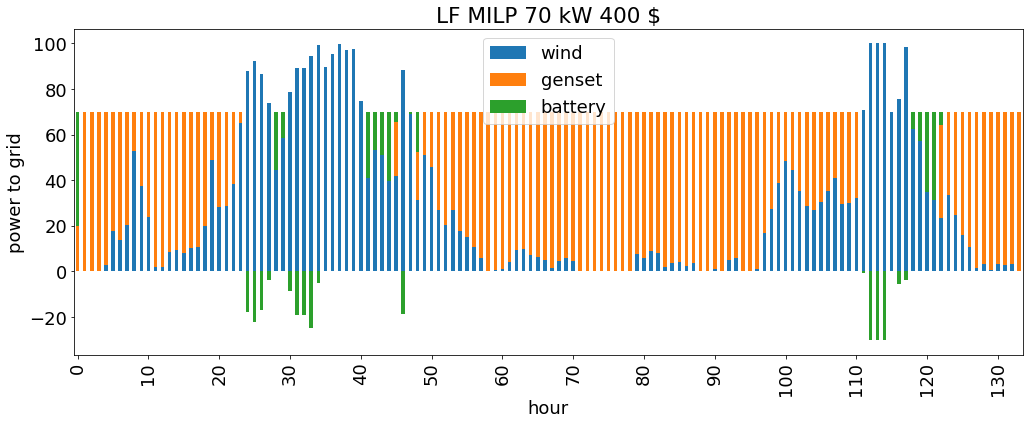
\includegraphics[scale=0.45]{/lf_70_400.png}
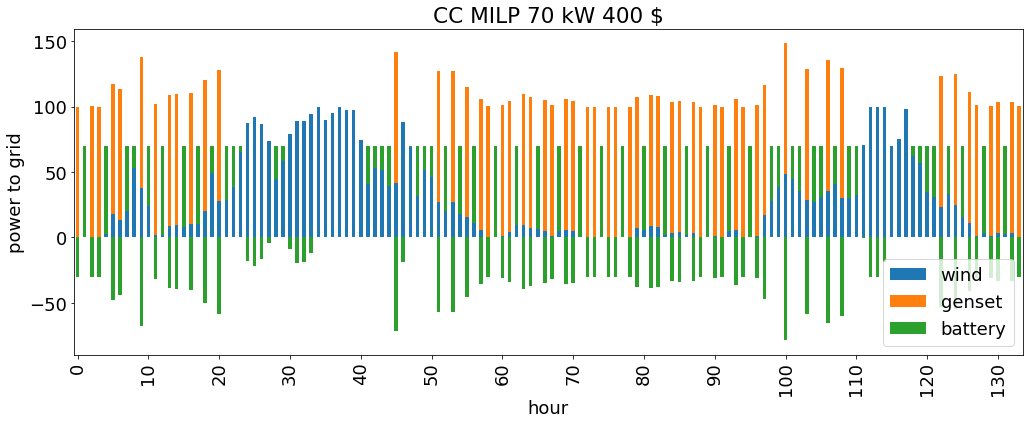
\includegraphics[scale=0.45]{/cc_70_400.png}
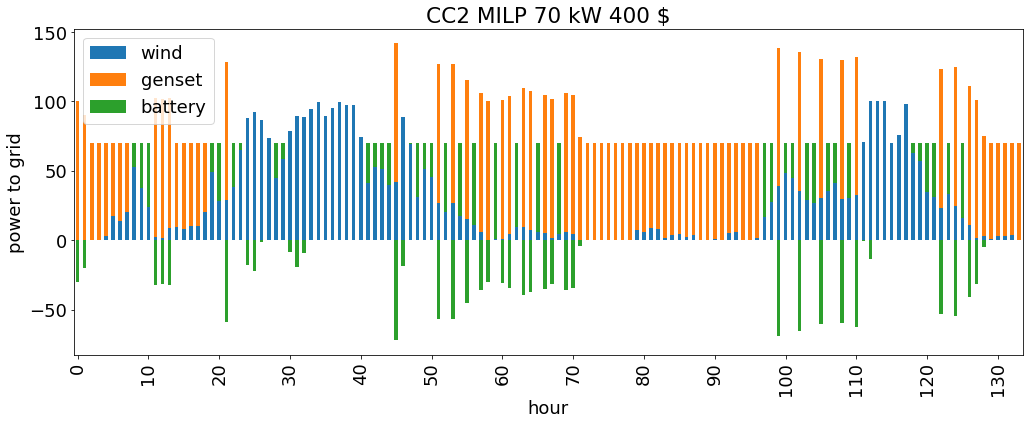
\includegraphics[scale=0.45]{/cc2_70_400.png}
\centering
\caption{Графики баланса мощности из численных экспериментов по сравнению стратегий планирования. Мощность нагрузки 70кВт, стоимость накопителя 1000\$/кВт ч. Положительные значения соответствуют генерации, отрицательные~---аккумуляции.}
\label{fig:res_70_400}
\end{figure}

\begin{figure}[H]
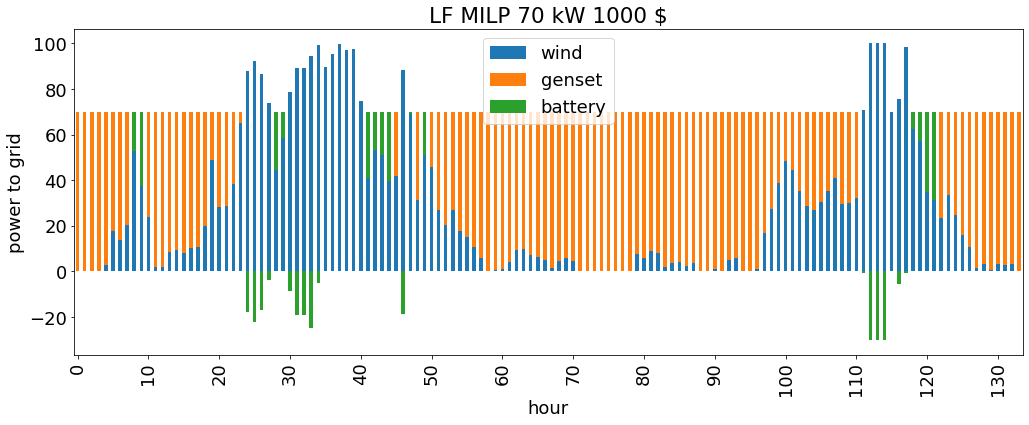
\includegraphics[scale=0.45]{/lf_70_1000.png}
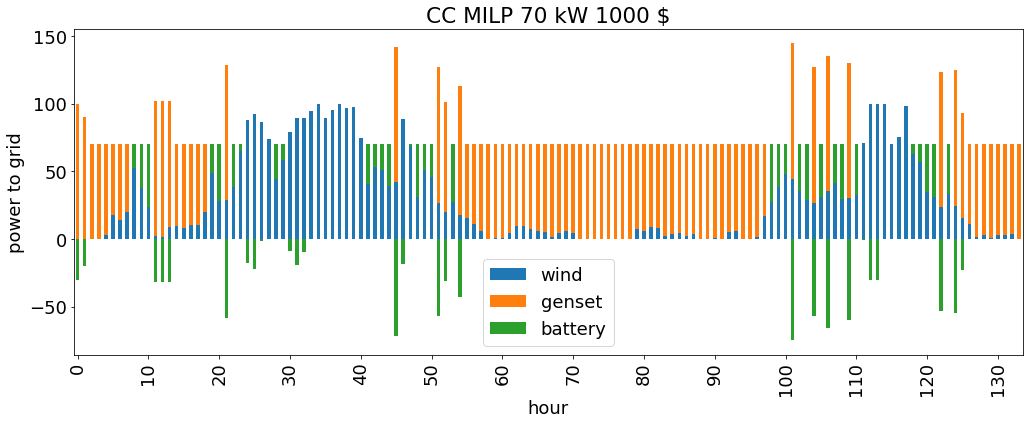
\includegraphics[scale=0.45]{/cc_70_1000.png}
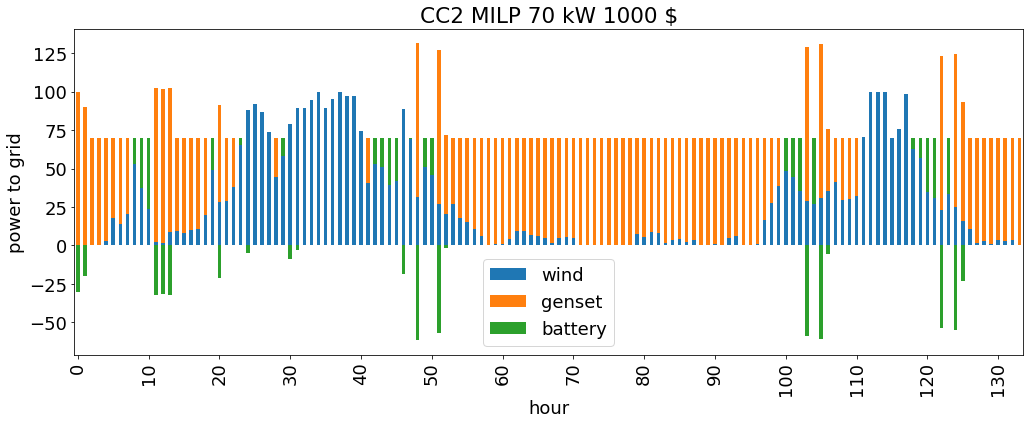
\includegraphics[scale=0.45]{/cc2_70_1000.png}
\caption{Графики баланса мощности из численных экспериментов по сравнению стратегий планирования. Мощность нагрузки 70кВт, стоимость накопителя 400\$/кВт ч. Положительные значения соответствуют генерации, отрицательные~---аккумуляции.}
\label{fig:res_70_1000}
\end{figure}

\begin{figure}[H]
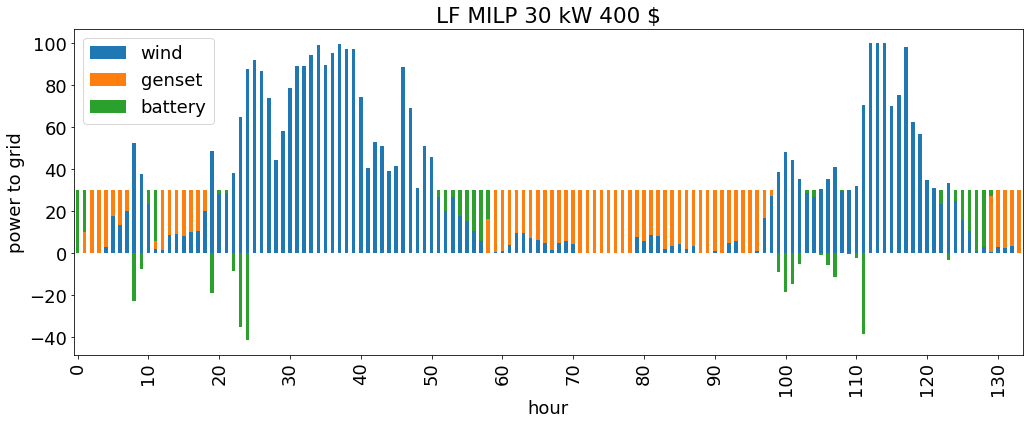
\includegraphics[scale=0.37]{/lf_30_400.png}
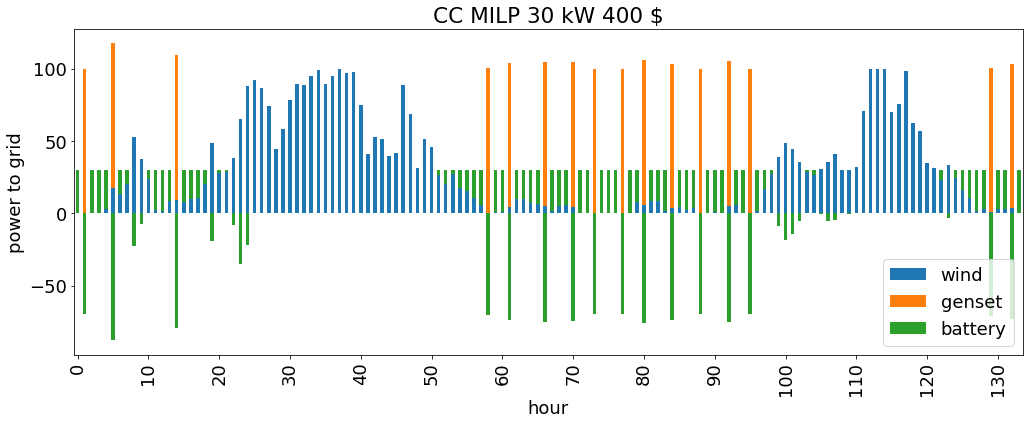
\includegraphics[scale=0.37]{/cc_30_400.png}
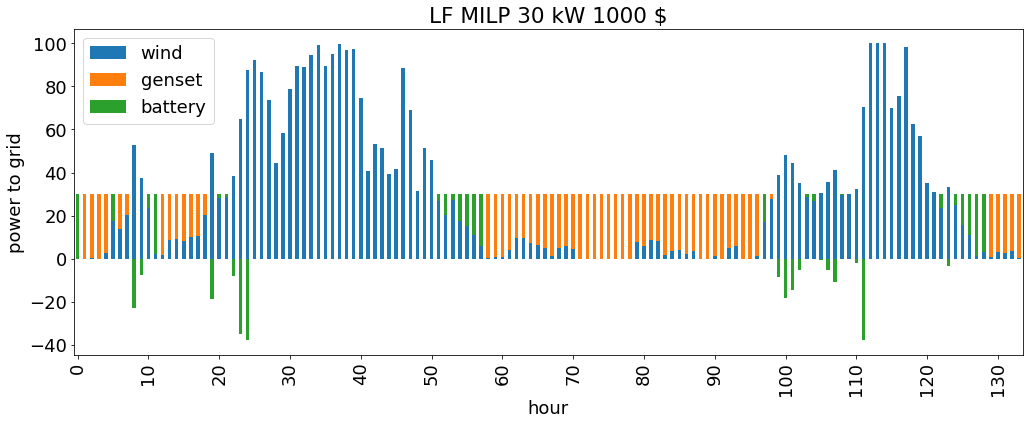
\includegraphics[scale=0.37]{/lf_30_1000.png}
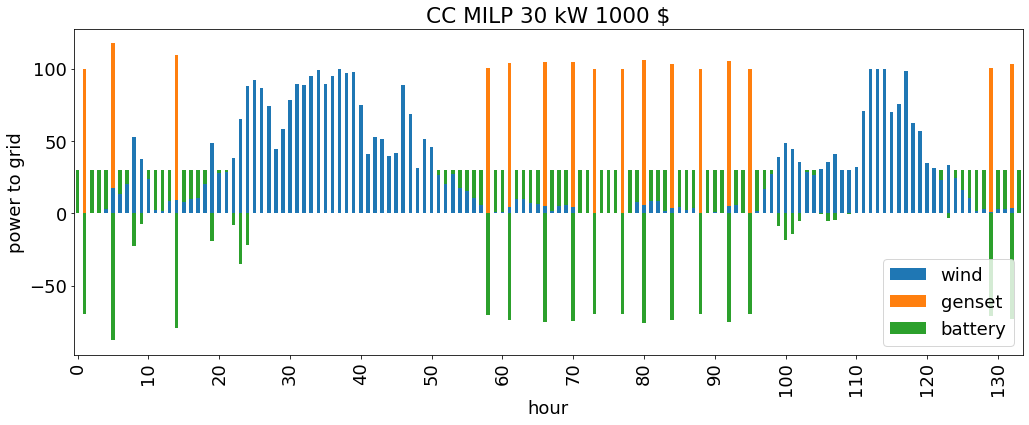
\includegraphics[scale=0.37]{/cc_30_1000.png}
\caption{Графики баланса мощности из численных экспериментов по сравнению стратегий планирования. Мощность нагрузки 70кВт. Положительные значения соответствуют генерации, отрицательные~---аккумуляции.}
\label{fig:res_30}
\end{figure}
